\chapterhead{4}{What Each Model Drops}{Two diagrams of one thing, two sets of answers}\label{ch4}

The same thing can have several models, and each one drops something different. A bus route has stops in a certain order, and the stops are some distance apart. A street map keeps the distances. A route diagram, the kind printed inside a bus, keeps only the order of the stops and spaces them evenly. Both are true to what they keep, and each can mislead about what it dropped.

\begin{center}
\sffamily\small\renewcommand{\arraystretch}{1.5}
\begin{tabular}{@{}p{3.4cm}p{3.7cm}p{3.7cm}@{}}
\toprule
\textbf{Model} & \textbf{What it keeps} & \textbf{What it drops}\\
\midrule
Street map to scale & distances and shape & the number of stops\\
Route diagram & order of stops & real distances\\
A model of any kind & what its maker needed & what they did not\\
\bottomrule
\end{tabular}
\end{center}

\begin{tryit}{Two diagrams of one walk}
Pick a walk, such as from home to a shop, with at least three stops or landmarks. Draw it twice: once as a map with the distances to scale, and once as a route diagram with the stops evenly spaced. Then ask both diagrams the same three questions.\par\medskip
\renewcommand{\arraystretch}{1.8}
\begin{tabular}{|p{4.0cm}|p{2.5cm}|p{2.5cm}|}
\hline
\textbf{Question} & \textbf{Map says} & \textbf{Diagram says}\\ \hline
Which two stops are closest? & & \\ \hline
How many stops after the first? & & \\ \hline
How far is it in all? & & \\ \hline
\end{tabular}
\end{tryit}

\begin{worked}{Practice numbers, not from a real route}
Four stops A, B, C, D. Real gaps: A to B 200~m, B to C 100~m, C to D 500~m. Total $200+100+500=800$~m.\\
Map at 1~cm to 100~m: gaps of 2, 1 and 5~cm, 8~cm in all. Route diagram: every gap drawn as 2~cm, 6~cm in all.\\
The map shows B and C are closest. The diagram shows three equal gaps and cannot say so.
\end{worked}

\begin{center}
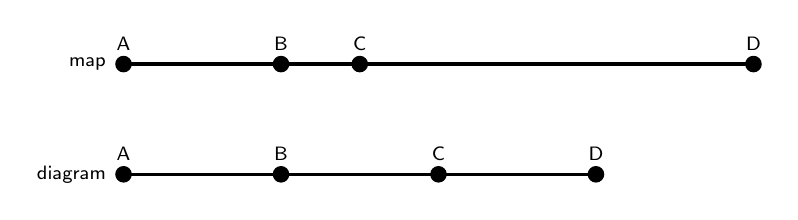
\begin{tikzpicture}[font=\sffamily\scriptsize]
  \node[left] at (-0.1,1.0) {map};
  \draw[line width=1.2pt] (0,1.0) -- (8,1.0);
  \foreach \x/\l in {0/A,2/B,3/C,8/D}{\fill (\x,1.0) circle (3pt); \node[above] at (\x,1.05) {\l};}
  \node[left] at (-0.1,-0.4) {diagram};
  \draw[line width=1.2pt] (0,-0.4) -- (6,-0.4);
  \foreach \x/\l in {0/A,2/B,4/C,6/D}{\fill (\x,-0.4) circle (3pt); \node[above] at (\x,-0.35) {\l};}
\end{tikzpicture}
\end{center}

\begin{multix}[hmm]\multixbot[hmm]\tcblower
The diagram shows the stops evenly spaced, so they are all the same distance apart. I trust drawings very much. Should I?
\end{multix}

\trust{We asked both diagrams the same three questions and compared each answer with the real distances.}
{It showed which question each diagram can answer: the map for distance, the diagram for order and count.}
{Anything neither diagram kept, such as hills, traffic or how long the walk takes.}

\begin{keepbox}
We turned one route into two diagrams. \textbf{We kept} \wline[3.4cm] \textbf{and we set aside} \wline[3.4cm].
\end{keepbox}

\clearpage

\begin{puzzle}{Add up}
Real gaps are 200, 100 and 500~m. Total \wline[1.6cm]~m. At 1~cm to 100~m the map is \wline[1.6cm]~cm long.
\end{puzzle}

\begin{puzzle}{Which diagram?}
Write M for the map, R for the route diagram or X if neither can answer.\\
(a) how far from A to D \wline[1cm] \quad (b) how many stops after A \wline[1cm] \quad (c) are there steep hills \wline[1cm]
\end{puzzle}

\begin{puzzle}{Equal gaps?}
On the route diagram C to D looks as far as B to C. In real life it is how many times farther? \wline[1.6cm]
\end{puzzle}

\begin{puzzle}{Kept and dropped}
List one thing the route diagram keeps and one it drops. \wline[6cm]
\end{puzzle}

\begin{puzzle}{Model or real}
Write M for model and R for real thing.\\
(a) the route diagram \wline[1cm] \quad (b) the street \wline[1cm] \quad (c) the map \wline[1cm]
\end{puzzle}

\clearpage

\begin{puzzle}{A tourist on foot}
Which would you give a tourist who must walk, the map or the diagram? \wline[2cm] Why? \wline[4cm]
\end{puzzle}

\begin{puzzle}{A bus passenger}
Which would you give a passenger who counts stops? \wline[2cm] Why? \wline[4cm]
\end{puzzle}

\begin{puzzle}{Draw the circles}
One street goes into two circles, a map and a diagram. Write one thing each keeps.
\begin{center}
\begin{tikzpicture}
  \node[bigcir,minimum size=2.2cm] (a) at (0,0) {}; \node[font=\sffamily\scriptsize] at (0,0) {street};
  \node[cir,minimum size=1.5cm] (b) at (4,0.9) {}; \node[cir,minimum size=1.5cm] (c) at (4,-0.9) {};
  \draw[popA] (a) -- node[above,note] {map} (b); \draw[popA] (a) -- node[below,note] {diagram} (c);
\end{tikzpicture}
\end{center}
\end{puzzle}

\begin{puzzle}{Wrap}
A student wrote ``The diagram is the better model.'' Wrap it with a better claim. \wline[6cm]
\end{puzzle}

\begin{puzzle}{Design two}
Choose something with parts, like a school or a body. Say what two diagrams of it would each drop. \wline[6cm]
\end{puzzle}
\clearpage

\thispagestyle{fancy}
\subhead{Two diagrams}
Draw your own walk both ways. Label each stop.\par\medskip
\begin{tikzpicture}\draw[ink!70,line width=1pt,rounded corners=3pt] (0,0) rectangle (11.4,3.6);\node[anchor=north west,font=\sffamily\small] at (0.1,3.5) {Map, drawn to scale};\end{tikzpicture}\par\medskip
\begin{tikzpicture}\draw[ink!70,line width=1pt,rounded corners=3pt] (0,0) rectangle (11.4,3.6);\node[anchor=north west,font=\sffamily\small] at (0.1,3.5) {Route diagram, stops evenly spaced};\end{tikzpicture}

\vspace{8pt}
Which question did the map answer that the diagram could not? \wline[3cm]\\[10pt]
Which question did the diagram answer more easily? \wline[3cm]
\clearpage
